\documentclass[a4paper, 14pt]{extarticle}
\usepackage[russian]{babel}
\usepackage[T1]{fontenc}
\usepackage{fontspec}
\usepackage{indentfirst}
\usepackage{enumitem}
\usepackage{graphicx}
\usepackage[
  left=20mm,
  right=10mm,
  top=20mm,
  bottom=20mm
]{geometry}
\usepackage{parskip}
\usepackage{titlesec}
\usepackage{xurl}
\usepackage{hyperref}
\usepackage{float}
\usepackage[
  figurename=Рисунок,
  labelsep=endash,
]{caption}
\usepackage[outputdir=build, newfloat]{minted}
\usepackage{multirow}
\usepackage{array}
\usepackage{tabularx}

\hypersetup{
  colorlinks=true,
  linkcolor=black,
  filecolor=blue,
  urlcolor=blue,
}

\renewcommand*{\labelitemi}{---}
\setmainfont{Times New Roman}
\setmonofont{JetBrains Mono}[
  SizeFeatures={Size=11},
]

\newenvironment{code}{\captionsetup{type=listing}}{}
\SetupFloatingEnvironment{listing}{name=Листинг}

\setminted{
  fontsize=\footnotesize,
  framesep=0mm,
}

\captionsetup{width=\textwidth,justification=centering}
\captionsetup[table]{singlelinecheck=off,justification=justified}

\newcolumntype{L}[1]{>{\raggedright\let\newline\\\arraybackslash\hspace{0pt}}m{#1}}
\newcolumntype{C}[1]{>{\centering\let\newline\\\arraybackslash\hspace{0pt}}m{#1}}
\newcolumntype{R}[1]{>{\raggedleft\let\newline\\\arraybackslash\hspace{0pt}}m{#1}}

\setlength{\parskip}{6pt}

\setlength{\parindent}{1cm}
\setlist[itemize]{itemsep=0em,topsep=0em,parsep=0em,partopsep=0em,leftmargin=2.0cm}
\setlist[enumerate]{itemsep=0em,topsep=0em,parsep=0em,partopsep=0em,leftmargin=2.0cm}

\renewcommand{\thesection}{\arabic{section}.}
\renewcommand{\thesubsection}{\thesection\arabic{subsection}.}
\renewcommand{\thesubsubsection}{\thesubsection\arabic{subsubsection}.}

\titleformat{\section}{\normalfont\bfseries}{\thesection}{0.5em}{}
\titleformat{\subsection}{\normalfont\bfseries}{\thesubsection}{0.5em}{}

\titleformat*{\section}{\normalfont\bfseries}
\titleformat*{\subsection}{\normalfont\bfseries}

\linespread{1.5}
\renewcommand{\baselinestretch}{1.5}
\begin{document}

\begin{titlepage}
  \vspace{0pt plus2fill}
  \noindent

  \vspace{0pt plus6fill}
  \begin{center}
    Санкт-Петербургский национальный исследовательский университет
    информационных технологий, механики и оптики

    \vspace{0pt plus2fill}

    Факультет инфокоммуникационных технологий

    Направление подготовки 11.03.02

    \vspace{0pt plus2fill}

    Практическая работа №6

    \vspace{0pt plus1fill}

    Трансляция адресов (NAT) в Cisco Packet Tracer

  \end{center}

  \vspace{0pt plus7fill}
  \begin{flushright}
    Выполнил: \\
    Швалов Даниил Андреевич

    Группа: К33211

    Проверил: \\
    Харитонов Антон
  \end{flushright}

  \vspace{0pt plus2fill}
  \begin{center}
    Санкт-Петербург

    2023
  \end{center}
\end{titlepage}

\setcounter{page}{2}

\section{Введение}

\textbf{Цель работы}: закрепить понимание принципов работы NAT, а также
сформировать начальные навыки в конфигурировании NAT и Firewall в Cisco Packet
Tracer.

\section{Ход работы}

По заданию необходимо заменить коммутатор 3-го уровня на маршрутизатор, а также
добавить еще один маршрутизатор и сервер. После добавления всех необходимых
устройств получилась схема, изображенная на рис. \ref{fig:scheme}.

\begin{figure}[H]
  \centering
  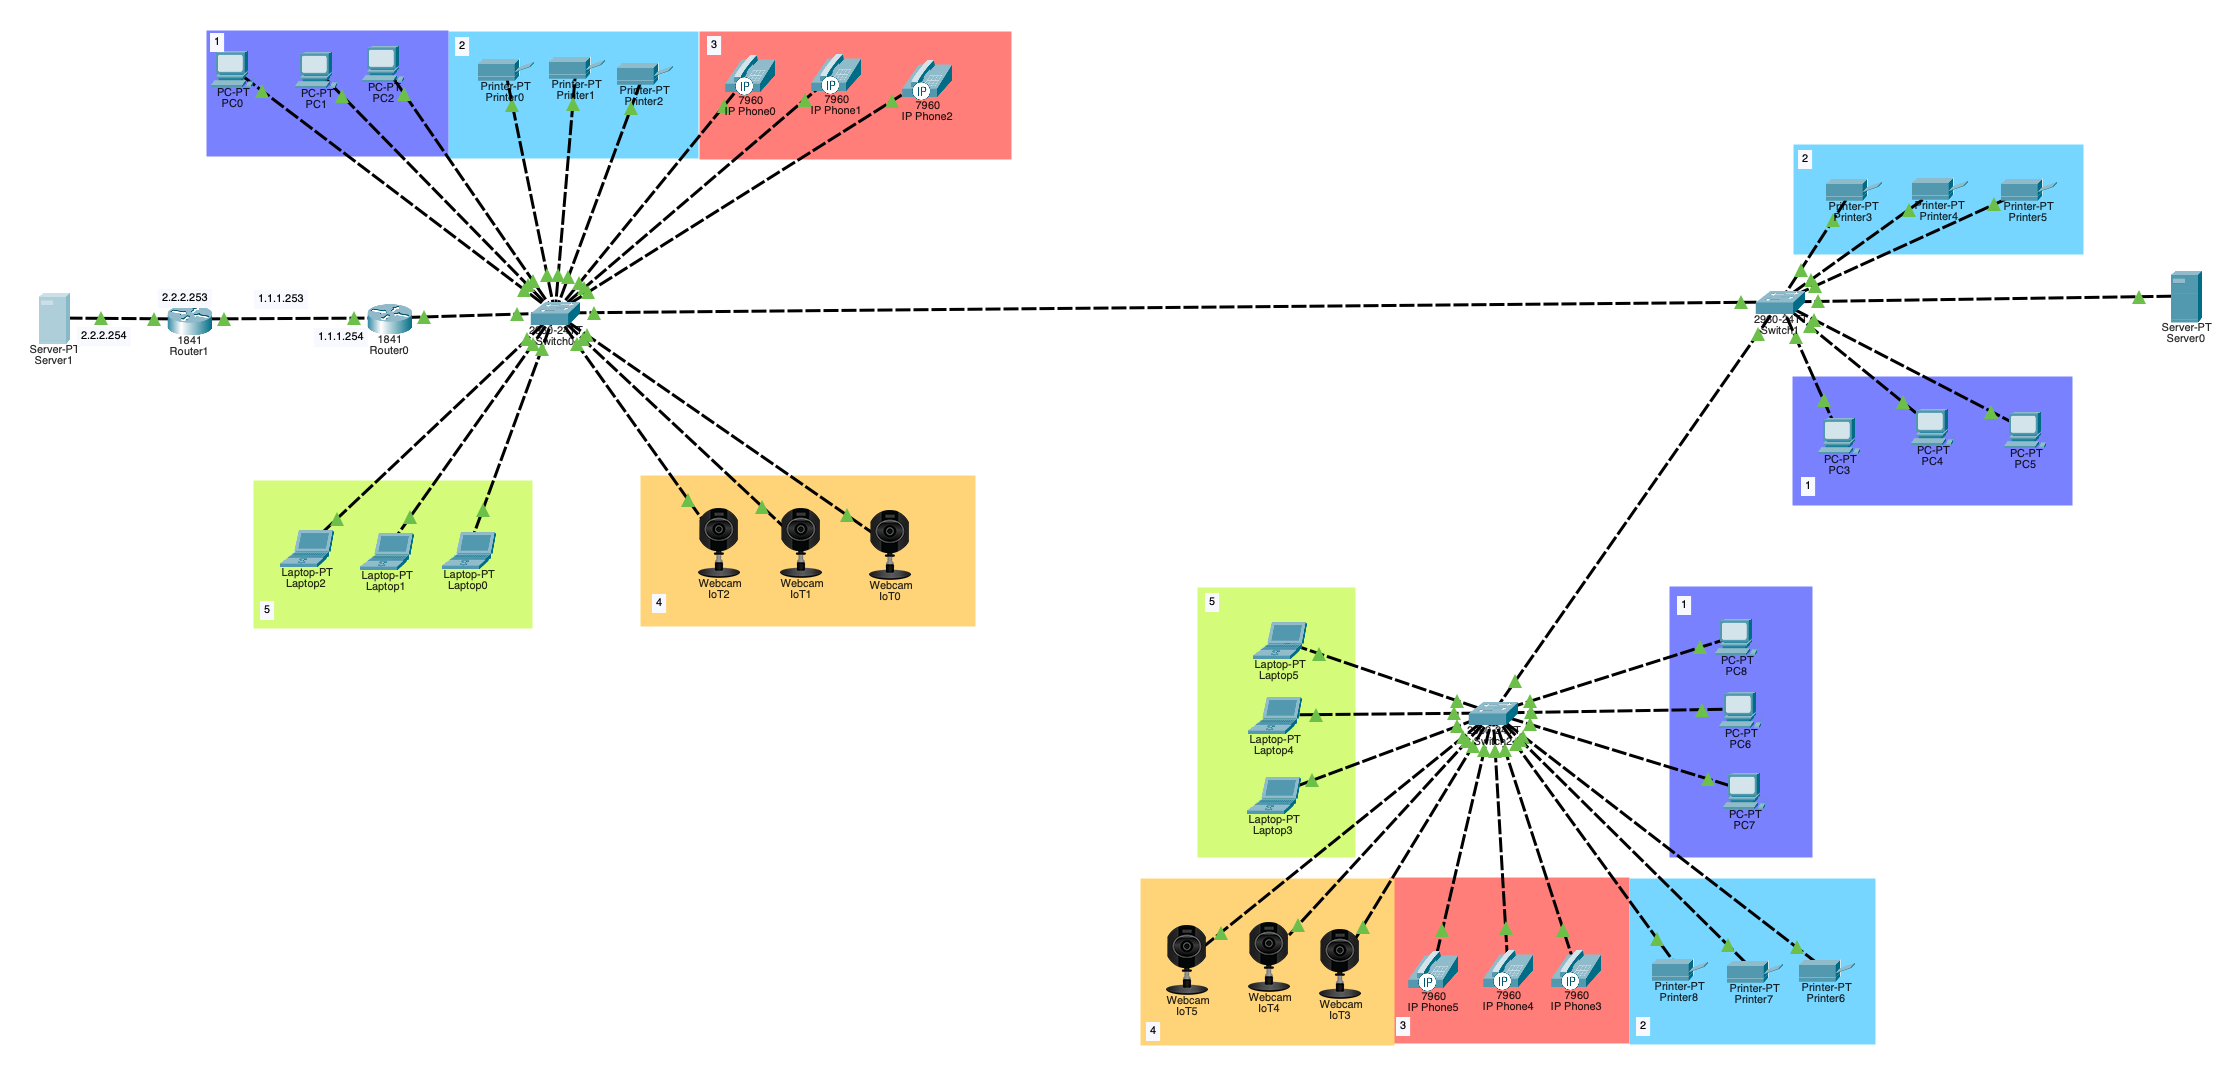
\includegraphics[width=\textwidth]{images/scheme.png}
  \caption{Схема сети}
  \label{fig:scheme}
\end{figure}

Поскольку ранее VLAN был настроен на коммутаторе 3-го уровня, после замены
коммутатора маршрутизатором его также необходимо было настроить. Для этого с
помощью следующих команд были добавлены все существующие VLAN в базу данных:
\begin{minted}{text}
  vlan database
  vlan 10 name VLAN-10
  vlan 20 name VLAN-20
  vlan 30 name VLAN-30
  vlan 40 name VLAN-40
  vlan 50 name VLAN-50
  vlan 60 name VLAN-50
\end{minted}

Затем необходимо было создать под-интерфейсы для каждого из VLAN, и назначить на
каждый из них IP-адрес. Далее показан пример настройки под-интерфейса для
первого VLAN:
\begin{minted}{text}
  int fa 0/0.10
  encapsulation dot1Q 10
  ip address 10.10.0.254 255.255.255.0
\end{minted}

Так как теперь сервер больше не выступает в качестве DHCP-сервера, необходимо
настроить DHCP-сервер на маршрутизаторе. Для каждого VLAN был создан свой набор
IP-адресов в соответствии с предыдущими лабораторными работами. Следующие
команды были использованы для настройки адресов первого VLAN:
\begin{minted}{text}
  ip dhcp pool VLAN-10
  network 10.10.0.0 255.255.255.0
  default-router 10.10.0.254
\end{minted}

После этого, в соответствии с заданием, необходимо было настроить IP-адреса на
портах двух добавленных маршрутизаторов. На маршрутизаторе, который связан с
локальной сетью, были выполнены следующие команды для настройки PAT:
\begin{minted}{text}
  int fa0/0.10
  ip nat inside
  int fa0/0.50
  ip nat inside
  int fa0/0.60
  ip nat inside
  int fa0/1
  ip nat outside
\end{minted}
Также на интерфейсе FastEthernet0/1 был настроен IP-адрес:
\begin{minted}{text}
  int fa0/1
  ip address 1.1.1.254 255.255.255.252
\end{minted}
и был прописан узел по умолчанию с помощью команды \texttt{ip route}:
\begin{minted}{text}
  ip route 0.0.0.0 0.0.0.0 1.1.1.253
\end{minted}

Далее на первом маршрутизаторе был создан access-list, который определяет какой
трафик должны пропускать через NAT. Для этого использовались следующие команды:
\begin{minted}{text}
  ip access-list standard NAT
  permit 10.10.0.0 0.0.0.255
  permit 10.50.0.0 0.0.0.255
  permit 10.60.0.0 0.0.0.255
\end{minted}
После чего access-list был применен для интерфейса FastEthernet0/0:
\begin{minted}{text}
  ip nat inside source list NAT int fa0/0 overload
\end{minted}

На втором маршрутизаторе были настроены адреса интерфейсов:
\begin{minted}{text}
  int fa0/0
  ip address 2.2.2.253 255.255.255.252
  int fa0/1
  ip address 1.1.1.253 255.255.255.252
\end{minted}

В итоге получилась схема, изображенная на рис. \ref{fig:ip}.

\begin{figure}[H]
  \centering
  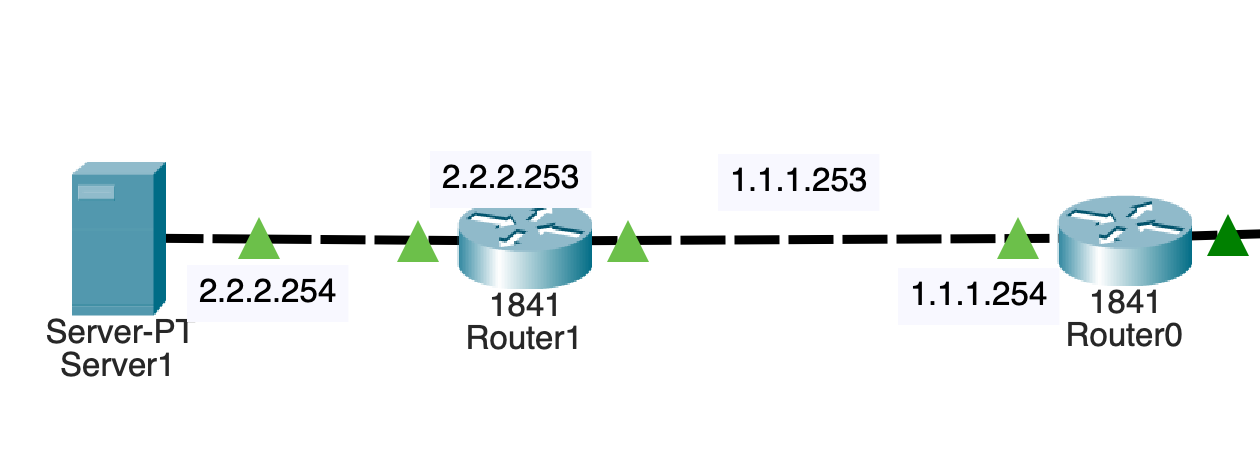
\includegraphics[width=\textwidth]{images/ip.png}
  \caption{Схема IP-адресов маршрутизаторов}
  \label{fig:ip}
\end{figure}

Для проверки работы правил NAT было сделано несколько тестовых запросов, после
чего была выполнена команда
\begin{minted}{text}
  show ip nat translations
\end{minted}
результат которой изображен на рис. \ref{fig:nat}.

\begin{figure}[H]
  \centering
  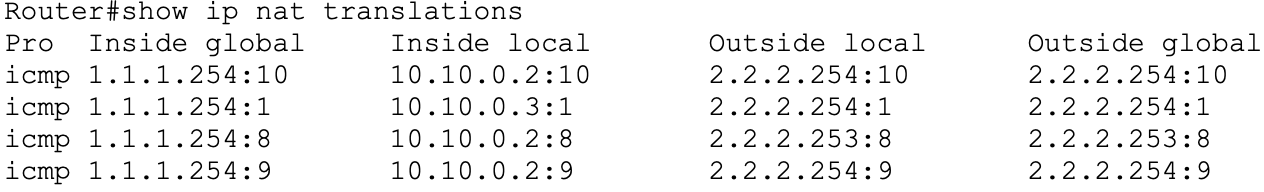
\includegraphics[width=\textwidth]{images/nat.png}
  \caption{Результат преобразования адресов}
  \label{fig:nat}
\end{figure}

Для того, чтобы локальный сервер был доступен из-вне, необходимо настроить
проброс портов с помощью следующей команды:
\begin{minted}{text}
  ip nat inside source static tcp 10.60.0.1 80 1.1.1.254 80
\end{minted}

После этого локальный сервер будет доступен с другого сервера из Интернета. На
рис. \ref{fig:website} показан пример веб-страницы, которую получает
пользователь при запросе по адресу 1.1.1.254.

\begin{figure}[H]
  \centering
  
\includegraphics[width=0.7\textwidth]{images/website.png}
  \caption{Веб-страница локального сервера}
  \label{fig:website}
\end{figure}

\section{Заключение}

В ходе выполнения лабораторной работы я закрепил понимание принципов работы NAT,
а также сформировал начальные навыки в конфигурировании NAT и Firewall в Cisco
Packet Tracer.

\end{document}
